%&pdflatex
\documentclass[preprint,3p,review,authoryear,10pt]{elsarticle}

\usepackage{graphicx}
\usepackage{natbib}
\usepackage{setspace}
\usepackage{multirow}
\usepackage{booktabs}
\usepackage[T1]{fontenc}
%\setlength{\parindent}{0in}
\usepackage{times}
\usepackage[british]{babel}
\usepackage{algorithm}
\usepackage{algorithmic} \renewcommand{\algorithmicrequire}{\textbf{Given:}} \renewcommand{\algorithmicensure}{\textbf{Returns:}}
\usepackage{amsfonts}
\usepackage{mathrsfs}
\usepackage{amssymb}
\usepackage{amsmath}
\usepackage{mathtools}
\renewcommand \thesection{\arabic{section}}
\usepackage[caption=false]{subfig}
\usepackage[compact]{titlesec}
\usepackage{soul}
\usepackage{textcomp}
\usepackage[section]{placeins}
\usepackage{url}
\usepackage{xspace}
\usepackage{lineno}
\usepackage{cleveref}

%Added by Diarmid
\usepackage{siunitx}

% % new commands
\newcommand{\I}{\mathcal{I}}
\DeclareMathOperator*{\any}{any}
\DeclareMathOperator*{\all}{all}

\newcommand{\ddt}[1]{\frac{\partial #1}{\partial t}}
\newcommand{\ddx}[1]{\frac{\partial #1}{\partial x}}

%% for annotating paper for TODO notes etc.  Comment this out and
%% uncomment alternative for final version
\newcommand{\sol}[1]{\footnote{#1}\marginpar{\fbox{\thefootnote}}}
%\newcommand{\esf}[1]{}

\journal{Computers \& Chemical Engineering}

\begin{document}
\linenumbers
\begin{frontmatter}

\title{The importance of fidelity in the scheduling of Redox Flow Batteries.}


\author{D. Roberts }
\author[]{S. Brown \corref{cor_author}}
\ead{s.f.brown@sheffield.ac.uk}

\address{Department of Chemical and Biological Engineering, The University of Sheffield, Sheffield S10 2TN}


\cortext[cor_author]{Corresponding author}

\begin{abstract}
Redox Flow Battery (RFB) systems are promising technologies for the multi-hour electrical energy storage that would be necessary in a future low carbon emission UK electrical grid based on wind and solar power. In order to perform techno-economic analyses (TEA) on these systems, it is necessary to calculate potential revenue for realistic applications, ideally under optimal operation (scheduling). In the present work, a novel schedule optimisation framework is introduced in which coulombic and voltaic components are separated, and the problem variablised in terms of current-density rather than power. This approach allows the expression of ohmic losses as a convex quadratic function of current-density in the objective function while maintaining all linear constraints. The resultant non-linear problem is more readily solvable than previous expressions in terms of power. It is demonstrated for an arbitrage application involving a vanadium RFB that the consideration of variable voltaic losses results in a significant improvement to the accuracy of revenue estimation when compared to the typical linear programming approach, where a fixed efficiency is assumed. The framework allows the removal of the assumption of a representative fixed open-cell voltage, which further improves revenue estimation, at the cost of computability. In a third case study, the framework allows a linear constraint on the working cell-voltage, resulting in current-density restriction at high state of charge (SOC) in order to avoid hydrogen and oxygen evolution. This feature would be relevant for the optimisation of Li-ion battery scheduling, where voltage is a very important consideration. The introduced framework is intended to assist technical optimisation of future RFB systems, for example in determining the optimum pump or cooling system size. The framework allows product optimisation in terms of revenue under optimal scheduling against a price signal (rather than metrics such as system cost, or lifetime cost per unit energy throughput as in previous works).

\end{abstract}

\begin{keyword}
Redox flow Battery \sep Optimisation \sep Non-linear Programming \sep Techno-Economic Analysis \sep Scheduling \sep VRFB  
%% keywords here, in the form: keyword \sep keyword

%% MSC codes here, in the form: \MSC code \sep code
%% or \MSC[2008] code \sep code (2000 is the default)

\end{keyword}

\end{frontmatter}

% \linenumbers

%% main text
\section{Introduction}
\label{sec:Intro}
The  growing deployment of intermittent renewable power sources \sol{you need numbers here to underline how important this is, i.e. what percentage of energy, around the world, is now renewable} such as wind and solar in industrialised nations in order to substitute fossil fuel power is a key driver of research into the development and applications of battery energy storage systems \sol{why? what does it do? the argument needs to highlight the properties that batteries have and why we think are important} (BESS). \sol{you need to pack in the references here, you mention research so we need references to know what they looked at...}

At present in the UK, the fluctuating output from these power sources is topped up to match demand primarily by varying the output of gas fired power plant \cite{DraxElectricInsights}. In order to meet the strict CO\textsubscript{2} emissions targets for the UK electrical supply by 2050, and bearing in mind that nuclear power capacity is not predicted to grow until after 2030 \cite{FES2018}, it is probable that further multi-hour energy storage will be required to displace gas plant from the role of balancing.  Within the UK electrical market, the phasing out of gas power plants, likely via increments to the carbon price \sol{reference?}, to be replaced by intermittent generation would lead to high electrical prices where demand exceeds supply, and low (or negative) pricing where supply exceeds demand.

At present, revenue from arbitrage on the wholesale electrical price is not in itself sufficient to justify BESS investment, and the deployment of grid scale BESS is dominated by projects that have won contracts for short term stability services tendered by National Grid. For example, \SI{500}{\mega\watt} of BESS capacity won contracts for the T-4 2020/21 capacity market (CM) auction, and \SI{200}{\mega\watt} of BESS capacity won enhanced frequency response (EFR) contracts. The majority of successful BESS applicants for the EFR auction also have CM contracts. \sol{This is a bit parochial, the same is regarding BESS elsewhere (i.e. the big Tesla abttery). We need to widen the story out to make the paper relevant outside the UK}

However, due to concerns that the average storage duration (i.e. energy to power ratio) of the BESS contracted for CM is shorter than the \SI{2}{\hour} that a stress event may last for, National Grid recently applied derating factors according to the energy to power ratio. Hence, a system rated at \SI{1}{\mega\watt}/\SI{2}{\mega\watt\hour} would only receive capacity payments for \SI{0.68}{\mega\watt} in the 2018/19 T-1 auction, and \SI{0.65}{\mega\watt} in the 2021/22 T-4 auction. The derating factor is relaxed to 0.96 for systems rated for 4+ hours of discharge \cite{NGDeratingFactors}. 

This development disfavours the power-centric Li-ion systems that previously won the majority of EFR contracts (Cite please) and favours redox flow battery (RFB) systems, where the incremental cost of energy capacity is low, and systems are typically specified with a 3-6 \si{\hour} energy to power ratio. 

In order to quantify the economic merits of RFB systems in comparison to other BESS, it is necessary to perform techno-economic analyses (TEA) for realistic applications. TEA should involve optimisation of the operation of a BESS to maximise revenue (or minimise costs). This should be done at various energy and power ratings (as these are decoupled in a non-hybrid RFB) to find the global optimum, as described by \cite{Oudalov2007}. The optimisation of operation requires determining the schedule, that is, the power output of the battery in each sub-period that maximises benefit without violating energy conservation.

For the optimisation of arbitrage revenue, the linear programming (LP) approach typically involves the maximisation of the objective function for revenue. Linear programming is an efficient problem formulation, as the optimum value for each variable will either lie at the maximum or minimum of a permitted value, making a search of the interior unnecessary.

Variants of the above formulation have been used to calculate the revenue or avoided costs due to RFB systems in various applications. For example, \cite{Hu2010} optimised the schedule of a VRFB and a poly-sulphide bromine RFB in order to maximise arbitrage revenue on the Danish day ahead electrical spot market. As the optimisation was to be performed daily, the SOC is constrained to return to 0 at the end of each \SI{24}{\hour} period.

\cite{Johnston2015} used a LP formulation to optimise the scheduling of a VRFB installed at a wind farm. The objective was to maximise revenue on the wholsesale electrical market while satisfying the frequency response obligations (constraints) of the wind installation\sol{what did they find?} . \cite{Vaca2017} looked at a similar application but compared the payback period for VRFB and supercapacitor installations with a hybrid system. In both studies, a cost of degradation in \pound per unit energy throughput was applied as a coefficient to ESS power variables in the objective function. This approach discourages the performance of arbitrage below a certain threshold price differential \sol{why is this note worthy?}.

A full system schedule optimisation problem was posed by \cite{Chen2012} to assess the benefit of a VRFB in a microgrid with a load, PV, wind and dispatchable micro-generation. When the micro-grid was isolated, the objective was to minimise the start-up and running costs of micro-generators used to back up the renewable power output. The authors used a mixed-integer LP (MILP) approach, where the innteger variables were used required to factor start-up costs, additional constraints were required to guarantee system reliability \sol{are these reliability constraints interesting?}. 

A significant simplification in all of the above studies is the assumption of a constant efficiency. In reality, the efficiency of any BESS is a function of the charge/discharge power (among other variables, such as SOC). In the above formulation, if efficiency were defined as a  function of power, it would be necessary to place this function on the denominator of the SOC increment term in the discharge expression in \Cref{eqn: Lit_Review_LP_SOC_Constraint_Example}.\sol{merge the previous and coming sentences to remove the reference to the equations} This complicates the problem as the constraint is now non-linear and non-quadratic. \cite{Nguyen2014} report a highly detailed nonlinear\sol{be consistent in you use of 'non-linear' or 'nonlinear'} model for the charge and discharge efficiency of a vanadium RFB. In a subsequent article (\cite{Nguyen2015}) this function was incorporated into the SOC expression of a schedule optimisation problem in the aforementioned fashion. Due to the complication of the SOC constraint, the authors employ a search approach with dynamic programming to break the problem down. This is more computationally intensive than the LP method, but the authors state that an optimum schedule may be found in an acceptable time-scale as the small number of variables and the presence of constraints limit the search space.

\cite{Sarker2017} also incorporated the dependency of efficiency on power in a scheduling problem (although applied to a Li-ion battery rather than a RFB). Quadratic terms are employed to relate losses to C-rate of charge and discharge. The presence of this quadratic function on the denominator of the discharge SOC increment term is avoided by redefining the discharge power variable as upstream of losses (rather than the power delivered to the grid). The discharge efficiency function is then moved from the SOC expression and multiplied by the discharge power variable in the objective function. The charge efficiency is left in the SOC expression (redefining the charge power variable in the same way would require dividing it by the quadratic charge efficiency term in the objective function). The problem therefore becomes convex (quadratic), but nonlinear in both objective function and constraint. The authors then employ a linear approximation technique\sol{does this need a reference}, and combine the efficiency treatment with a piece-wise linear treatment of degradation as a function of power, giving an overall mixed integer-linear programming problem (MILP). 

In this work, the schedule problem is formulated in terms of current-density rather than power, which allows the separation of coulombic and voltaic efficiency components. It will be shown that important constraints on the problem may be posed more readily in this form.\sol{you do more than this, you formulate this problem 3 times with increasing levels of complexity then apply each of these to a case study to compare their performance. You need to say this and be sure to say that this is all novel, otherwise it's not clear why the reviewers should be bothered}

This paper is organised as follows: Section \ref{sec:Model_Formulation} presents...\sol{complete this paragraph}

\section{Model formulation}
\label{sec:Model_Formulation}
\sol{describe what you're going to do here...}
\subsection{LP Problem in Current-Density Terms}
\label{Model_Formulation_LP_Reference_Current_Density_Terms}
The typical LP formulation for the scheduling problem uses an objective function which is formulated in terms of the power as \sol{give references}:

\begin{equation}
\label{eqn:Lit_Review_LP_Obj_Func}
R = \tau \sum_{t} (P_{Dis,t} - P_{Chg,t}) p_t
\end{equation}

where $P_{Dis,t}$ and $P_{Chg,t}$ represent the bounded variables discharge and charge power between the RFB and the rest of the system in period $t$, $\tau$ the time-step parameter (length of period $t$) and $p_t$ the parameter price of electrical energy in period $t$.

The state of charge (SOC) of the BESS is then defined by:

\begin{equation}
\label{eqn: Lit_Review_LP_SOC_Constraint_Example}
\begin{gathered}
SOC_t = SOC_{t-1} + \frac{\tau P_{Chg,t} \eta_{Chg}}{E_{BESS}} - \frac{\tau P_{Dis,t}}{E_{BESS}\eta_{Dis}} \\
\end{gathered}
\end{equation}

where $E_{BESS}$ is the parameter energy capacity and $\eta_{Chg}$ and $\eta_{Dis}$ are the charge and discharge energy efficiency parameters respectively. The SOC is at all times normally constrained to between a maximum of 1 and a minimum of 0, though a narrower window has also used \sol{reference}.

To re-pose this in terms of current-density, the power variable(s) with charge and discharge current-density variables.\sol{can you describe the relations that you've used here}

Current-density was chosen over current as the former is a scale-independent metric commonly used in the RFB literature. The use of current-density makes multiplication by stack area necessary to obtain absolute current, and multiplication by open-cell-volage (OCV) necessary to obtain power. Separate efficiencies representing voltaic and ohmic losses must now be specified, rather than the single energy efficiency term in \cref{eqn: Lit_Review_LP_SOC_Constraint_Example}. As current-density is defined based on the current at the RFB terminals, coulombic losses are dealt with upstream in \cref{eqn: Method_SOC_Tracker}. It is however necessary to incorporate voltaic losses in the objective function.  The objective function for revenue in period $Y$ (to be maximised) is defined by:


\begin{equation}
\label{eqn: Linear_Schedule_Objective_Function_Current_as_Variable}
R_{LP} = \frac{A.\tau OCV_{50\%}}{1\times 10^{6}}\sum_{t}p_{t}(I_{D, t}\sqrt{\bar\eta_{V}}(1 - l_{BOP}) - \frac{I_{C,t}}{\sqrt{\bar\eta_{V}}(1 - l_{BOP})}) \; \forall t \in Y
\end{equation}

where $I_{C,t}$ and $I_{D,t}$ are independent variables representing charge and discharge current density (\si{\ampere\per\square\meter}) respectively. $A$ is the stack area parameter (\si{\square\meter}), $\tau$ the timestep (\si{\hour}), $OCV_{50\%}$ the open cell voltage at 50\% state of charge (SOC) and $p_t$ the indexed electrical price parameter (\SI[sticky-per, bracket-unit-denominator = false]{}[\pounds]{\per\mega\watt\hour}). $\bar\eta_{V}$ is the representative round-trip voltaic efficiency. The  placement of the additional fractional balance of plant losses parameter $l_{BOP}$ reflects the assumption that balance of plant power consumption is primarily due to electrolyte pumping, and that pumping power is proportional to current. The validity of this assumption is discussed in \cref{analysis_of_assumptions}. 

The function describing SOC given in \cref{eqn: Lit_Review_LP_SOC_Constraint_Example} is now expressable in purely coulombic terms. This is done by replacing the power variables with current-density variables, the energy efficiency parameters with a coulombic efficiency parameter, and the energy capacity of the RFB with a coulombic capacity. The resultant function for the SOC at the end of sub-period $t$ is defined by:

\begin{equation}
\label{eqn: Method_SOC_Tracker}
SOC_t = SOC_{t-1} + \frac{A.\tau}{1000C}(I_{C,t}\sqrt{\eta_C} - \frac{I_{D,t}}{\sqrt{\eta_C}}) \; \forall t \in Y
\end{equation}

where $C$ is the coulombic capacity of the RFB (\si{\ampere\hour}). It is assumed that the coulombic efficiency $\eta_C$ does not vary with SOC or current-density, and that coulombic losses for charge and discharge are symmetrical. This assumption is discussed in \cref{analysis_of_assumptions}. 

The following constraints are applied to the list of SOC values generated by the above expression. Firstly the constraint on SOC range is formalised by:

\begin{equation}
\label{eqn: Method_Constraint_SOC_Range}
SOC_{min} \leq SOC_t \leq SOC_{max} \; \forall t \in Y
\end{equation}

where $SOC_{min}$ and $SOC_{max}$ are the minimum and maximum permitted SOC parameters.

So that the optimisation may be legitimately performed on consecutive periods of historical data (i.e. maintaining an energy balance) the SOC is required to return to 50\% at the end of each period. This constraint is formalised by:

\begin{equation}
\label{eqn: Method_Constraint_E_Conservation}
SOC_0 = SOC_n = 0.5
\end{equation}
where $n$ is the final sub-period in $Y$.

Finally, the current-density in and out of the RFB is constrained by:

\begin{equation}
\label{eqn: Method_Constraint_Ia}
I_{min} \leq I_{D,t}, \; I_{C,t} \leq I_{max} \; \forall t \in Y
\end{equation}

where $I_{min}$ and $I_{max}$ are the minimum and maximum permitted current-densities respectively.

\subsection{NLP treatment of voltaic losses}
\label{Model_Formulation_NLP_treatment_voltaic_losses}
A major simplification in the LP problem in terms of power is the assumption of a constant energy efficiency parameter. This assumption also applies to the LP problem in current-density terms introduced in \cref{Model_Formulation_LP_Reference_Current_Density_Terms}, although separate voltaic and coulombic efficiencies parameters are called for. In reality, ohmic (and pseudo-ohmic) over-potential is a linear function of current-density . The faradaic over-potential, which occurs when the circuit is closed, may be considered constant with respect to current-density (CITE article I used in CR). \cref{eqn: Linear_Schedule_Objective_Function_Current_as_Variable} was adapted to include these losses, by subtracting/adding the faradaic over-potential from/to the OCV during discharge/charge, and including the ohmic losses in the form of the classical $P_{Loss} = I^2R$ equation. This results in a nonlinear (NLP) objective function for revenue in period $Y$ defined by:

\begin{equation}
\label{eqn: Non-Linear_Schedule_Objective_Function_Current_as_Variable}
R_{NLP} = \frac{A.\tau}{1\times 10^{6}}\sum_{t}p_{t}(I_{D, t}(OCV_{50\%} - V_a)(1-l_{BOP}) - \frac{I_{C, t}(OCV_{50\%} + V_a)}{1-l_{BOP}} - (I_{D,t}^{2} + I_{C,t}^{2})ASR) \; \forall t \in Y
\end{equation}


where $V_a$ and $ASR$ are scalar parameters representing faradaic over-potential (\si{\volt}) and area specific resistance (\si{\ohm\square\meter}). The placement of $V_a$ and $ASR$ reflects an assumption of symmetry in voltaic losses between charge and discharge (discussed further in \cref{analysis_of_assumptions}). The objective function is subject to the same constraints as described in \cref{Model_Formulation_LP_Reference_Current_Density_Terms}.

Although non-linear, \cref{eqn: Non-Linear_Schedule_Objective_Function_Current_as_Variable} the objective function is convex (as it requires maximising a negative quadratic), hence a gradient based algorithmic solver is guaranteed to find the optimum from any starting point. 



Under the constant coulombic efficiency assumption \cref{eqn: Method_SOC_Tracker} is linear, and so by extension are the constraints in \cref{eqn: Method_Constraint_SOC_Range,eqn: Method_Constraint_E_Conservation}.  The overall formulation hence comprises a nonlinear objective function subject to linear constraints. This is an improvement over the formulations of losses expressed in power efficiency terms by \cite{Nguyen2015,Sarker2017}, both of which use non-linear SOC constraint expressions. According to \cite{Hart2017}

\textit{"In the context of nonlinear models, those with nonlinear objective functions are typically easier to optimize than models with nonlinear constraint expressions"}

The formulation also benefits from a consistent definition of the current-density variables in terms of flow between the terminals and the external system, unlike in \cite{Sarker2017}.

The NLP problem is based on an assumption of constant coulombic efficiency, which is discussed further in \cref{analysis_of_assumptions}.

\subsection{Functional Treatment of OCV}
\label{Model_Formulation_Functional_Treatment_OCV}
A simplification in the NLP problem introduced in \cref{Model_Formulation_NLP_treatment_voltaic_losses} is the use of a fixed OCV, ($OCV_{50\%}$) where OCV is in fact a function of SOC. If the OCV is linear with respect to SOC in the permitted SOC range (which, in the case of the system described by \cite{Reed2016} it is), and the RFB transfers as much energy below 50\% SOC as above it, then this assumption may be reasonable.
However, using the current-density formulation, it is possible to functionalise the relationship between OCV and SOC. The relationship between the average OCV and the average SOC in sub-period t is approximated by:

\begin{equation}
\label{eqn: OCV_vs_SOC}
OCV_t = a\frac{SOC_t + SOC_{t-1}}{2} + b 
\end{equation}

where $a$ and $b$ are system specific parameters.

Replacing $OCV_{50\%}$ with $OCV_t$ in \cref{eqn: Non-Linear_Schedule_Objective_Function_Current_as_Variable} and expanding $SOC_t$ and $SOC_{t-1}$ by \cref{eqn: Method_SOC_Tracker} results in an objective function (to be maximised) defined by:


\begin{equation}
    \label{eqn: NLP_true_OCV_long_form}
    \begin{split}
R_{NLP} = \frac{A.\tau}{1\times 10^{6}}\sum_{t}p_{t}(\\
(1-l_{BOP})I_{D, t}(a\frac{SOC_{t-1} + SOC_{t-2} + \frac{A.\tau}{1000C}(I_{C,t}\sqrt{\eta_C} - \frac{I_{D,t}}{\sqrt{\eta_C}} +  I_{C,t-1}\sqrt{\eta_C} - \frac{I_{D,t-1}}{\sqrt{\eta_C}})}{2} + b - V_a)\\ - \frac{1}{1-l_{BOP}}(I_{C, t}(a\frac{SOC_{t-1} +  SOC_{t-2} + \frac{A.\tau}{1000C}(I_{C,t}\sqrt{\eta_C} - \frac{I_{D,t}}{\sqrt{\eta_C}} + I_{C,t-1}\sqrt{\eta_C} - \frac{I_{D,t-1}}{\sqrt{\eta_C}})}{2} + b + V_a))\\ 
- (I_{D,t}^{2} + I_{C,t}^{2})ASR) \; \forall t \in Y
\end{split}
\end{equation}


This objective function is non-convex, due to the presence of bivariate quadratic terms  (e.g. $-I_{D,t}I_{C,t-1}$). However, it is possible to solve the problem by generating a positive semidefinite


\subsection{Cell Voltage Constraint}
\label{Model_Formulation_Constraint_Cell_Voltage}
It has so far been assumed that the RFB may accept the maximum charge current-density right up to the maximum permitted SOC. In reality this may result in the cell-voltage being too-high (overcharging, discussed further in \cref{Results_Cell_Voltage_Constraint}. An alternative charging approach (common for Li-ion batteries where high cell voltages pose safety concerns) is to switch to a constant voltage taper charge at high SOC, where the current declines until a cut-off value is reached. In the case of an RFB, the fixed losses described above would likely make taper charging uneconomical (see the low efficiency at low current-density reported by \cite{Nguyen2014}). Rather than globally adjust the maximum permitted charge current-density or SOC (which may lead to underestimation of revenue), the objective function in \cref{eqn: Non-Linear_Schedule_Objective_Function_Current_as_Variable} is made subject to a new linear constraint in terms of cell-voltage, defined by:
    
    \begin{equation}
\label{eqn: Cell_Voltage_Constraint}
OCV_t + V_a + I_{C,t}ASR \leq V_{max} \; \forall t \in Y
\end{equation}

Where $V_{max}$ is the maximum permitted cell-voltage. As $OCV_t$ is an averaged value of SOC in the sub-period $t$ (\cref{eqn: OCV_vs_SOC}), the accuracy of the model should improve as $\tau$ is reduced. A similar constraint could be implemented for discharge if required.

\subsection{RFB Specification}
\label{VRFB_specification}
The RFB is modelled here as a single cell. As the power output of a hypothetical RFB may be increased at the cost of efficiency, it is necessary to specify a rated efficiency when determining the stack area required for, say, a \SI{1}{\kilo\watt} system. This is formalised by:

\begin{equation}
\label{eqn: Rated_efficiency}
\eta_{DC} = \eta_{V,rated}\eta_{C}(1-l_{BOP})^2 = \eta_{rated}
\end{equation}

Where $\eta_V$ and $\eta_C$ are the round trip voltaic and coulombic efficiencies respectively. It is assumed that the one-way fractional balance of plant losses ($l_{BOP}$) are primarily due to electrolyte pumping, and that the pump runs on DC power.

The stack area (\si{\square\meter}) is calculated by:

\begin{equation}
\label{eqn: Simple_RFB_Cost_Model_Stack_Area}
A = \frac{P_{rated}}{I_{rated}V_0\sqrt{\eta_V}(1 - l_{BOP})}
\end{equation}

where $P_{rated}$ is the system power rating (\si{\watt}) and $I_{rated}$ is the current density (\si{\ampere\per\square\metre}) corresponding experimentally to coulombic and voltaic efficiencies that satisfy \Cref{eqn: Rated_efficiency}.

The coulombic capacity of the VRFB, required for the tracking of SOC in \Cref{eqn: Method_SOC_Tracker}, is calculated by:

\begin{equation}
\label{eqn: coulombic_capacity}
C = \frac{AI_{rated}r_{e:p}}{\sqrt{\eta_C}}
\end{equation}

Where $r_{e:p}$ is the specified energy to power ratio of the system. The presence of $\eta_C$ ensures there is sufficient chemical energy in the tank to cover coulombic losses upon discharge (square root after \cite{Darling2014}).


\section{Case Study}
\label{Case Study}

\subsection{The Application}
\label{Results_The_Application}
Pure price arbitrage on the day ahead N2EX electrical market was chosen as a case study, as the availability of future price information makes deterministic schedule optimisation relevant. Schedule optimisation was performed on 24h periods, with $\tau$ of 1h. The indexed price $p_t$ was parametrised using data obtained from the NordPool website \cite{NordPool2016}.

\subsubsection{The RFB}
\label{Model_Formulation_VRFB_Params}
\cite{Reed2016} studied various electrode flow architectures on a \SI{1}{\kilo\watt} VRFB system based on a \SI{50}{\micro\meter} Nafion NR212 membrane. In this case study, performance data were taken from the test of the highest performing stack architecture (IDD2s) at an electrolyte flow rate of 400 \si{\ml\per\minute} (per cell). This setup was tested at three current-densities: 1600, 2400 and 3200 \si{\ampere\per\square\meter}. At each test condition efficiency data were obtained as integrals over a cycle between 15\% and 85\% SOC. 

In the parametrisation of the VRFB for following case studies $P_{rated}$ was set at \SI{1}{\kilo\watt}, the energy to power capacity ratio $r_{e:p}$ was set at 4 and $\eta_{rated}$ was set at 75\%. $L_{BOP}$ was set at 0.02, based on a conservative interpretation of the pumping power data reported for a very similar system by \cite{Kim2013}. A coulombic efficiency ($\eta_C$) of 0.975 was derived as the average of the values reported by \cite{Reed2016} at the three current-densities tested, which only varied between 0.974 and 0.976.  For the chosen system  the overall energy efficiency requirement in \cref{eqn: Rated_efficiency} is satisfied when the voltaic efficiency $\eta_{V,rated}$ is 0.801, which corresponds (by linear interpolation) to a current-density ($I_{rated}$) of \SI{2188}{\ampere\per\square\meter}. $OCV_{50\%}$ was taken from \cite{Kim2011}, where the OCV of a chloride electrolyte was reported at 20\%, 50\% and 80\% SOC. Although a different electrolyte (based on a mixture of sulphuric acid and hydrochloric acid) was used in \cite{Reed2016}, OCV data have not been published.

\cref{tab:VRFB_Sizing_Params} summarises the parameter values used to represent the VRFB.

\begin{table}[!pht]
\captionsetup{font=normalsize}
\centering
\caption{Parameters describing VRFB in sizing process}
\label{tab:VRFB_Sizing_Params}
\begin{tabular}{ccccccc}
\hline
Param &  Value & Units &  Source \\
\hline
$P_{rated}$ & 1 & \si{\kilo\watt} & Arb.\\
$r_{e:p}$ & 4 & - & \multirow{2}{*}{Typical}\\
$\eta_{rated}$ & 0.75 & - \\
\hline
$\eta_{V,rated}$ & 0.801 & - &\multirow{3}{*}{\cite{Reed2016}}\\
$\eta_C$ & 0.975 & -\\
$I_{rated}$ & 2188 & \si{\ampere\per\square\meter} \\
\hline
$OCV_{50\%}$ & 1.46 & \si{\volt} & \cite{Kim2011}\\
$l_{BOP}$ & 0.02 & - & \cite{Kim2013}\\

\hline
\end{tabular}
\end{table}

\subsection{Implementation}
\label{Results_Implementation}
Each optimisation problem was posed using PYOMO within a Python loop for repeat solutions on 24h sets of data. The gurobi solver was called via the SolverFactory module. The script was run on a virtual machine (\cite{VirtualBox}) running Linux Mint, which was allocated 1024 MB RAM.


\subsection{NLP treatment of Voltaic Losses}
\label{Results_NLP_Treatment_Voltaic_losses}
In the first case study, the performance of the NLP formulation with functionalised voltaic losses (\cref{Model_Formulation_NLP_treatment_voltaic_losses}) was assessed by comparison to the LP formulation described in \cref{Model_Formulation_LP_Reference_Current_Density_Terms}. The LP objective function in \cref{eqn: Linear_Schedule_Objective_Function_Current_as_Variable} requires the assumption of a constant voltaic efficiency term $\bar\eta_{V}$. A value of 0.842 was applied, as this is the voltaic efficiency at the mid-point of the permitted current-density range (\SI{1600}{\ampere\per\square\meter}). The NLP formulation in \cref{eqn: Non-Linear_Schedule_Objective_Function_Current_as_Variable} requires values for area specific resistance ($ASR$) and Faradaic potential ($V_a$) in order to parametrise voltaic losses in the objective function. These were derived by multiplying $OCV_{50\%}$ by $1-\sqrt{\eta_V}$ to obtain an over-potential $\delta_v$ at the three current-density points in the experimental data (assuming losses are symmetrical in charge and discharge). $ASR$ was obtained as the gradient of the linear regression on this plot, and $V_a$ as the intercept at zero current-density.

\cref{fig:Va_ASR_Derivation} shows the regression of $\delta_V$ against current density for the data taken from \cite{Reed2016}.

\begin{figure}[!ht]
\centering
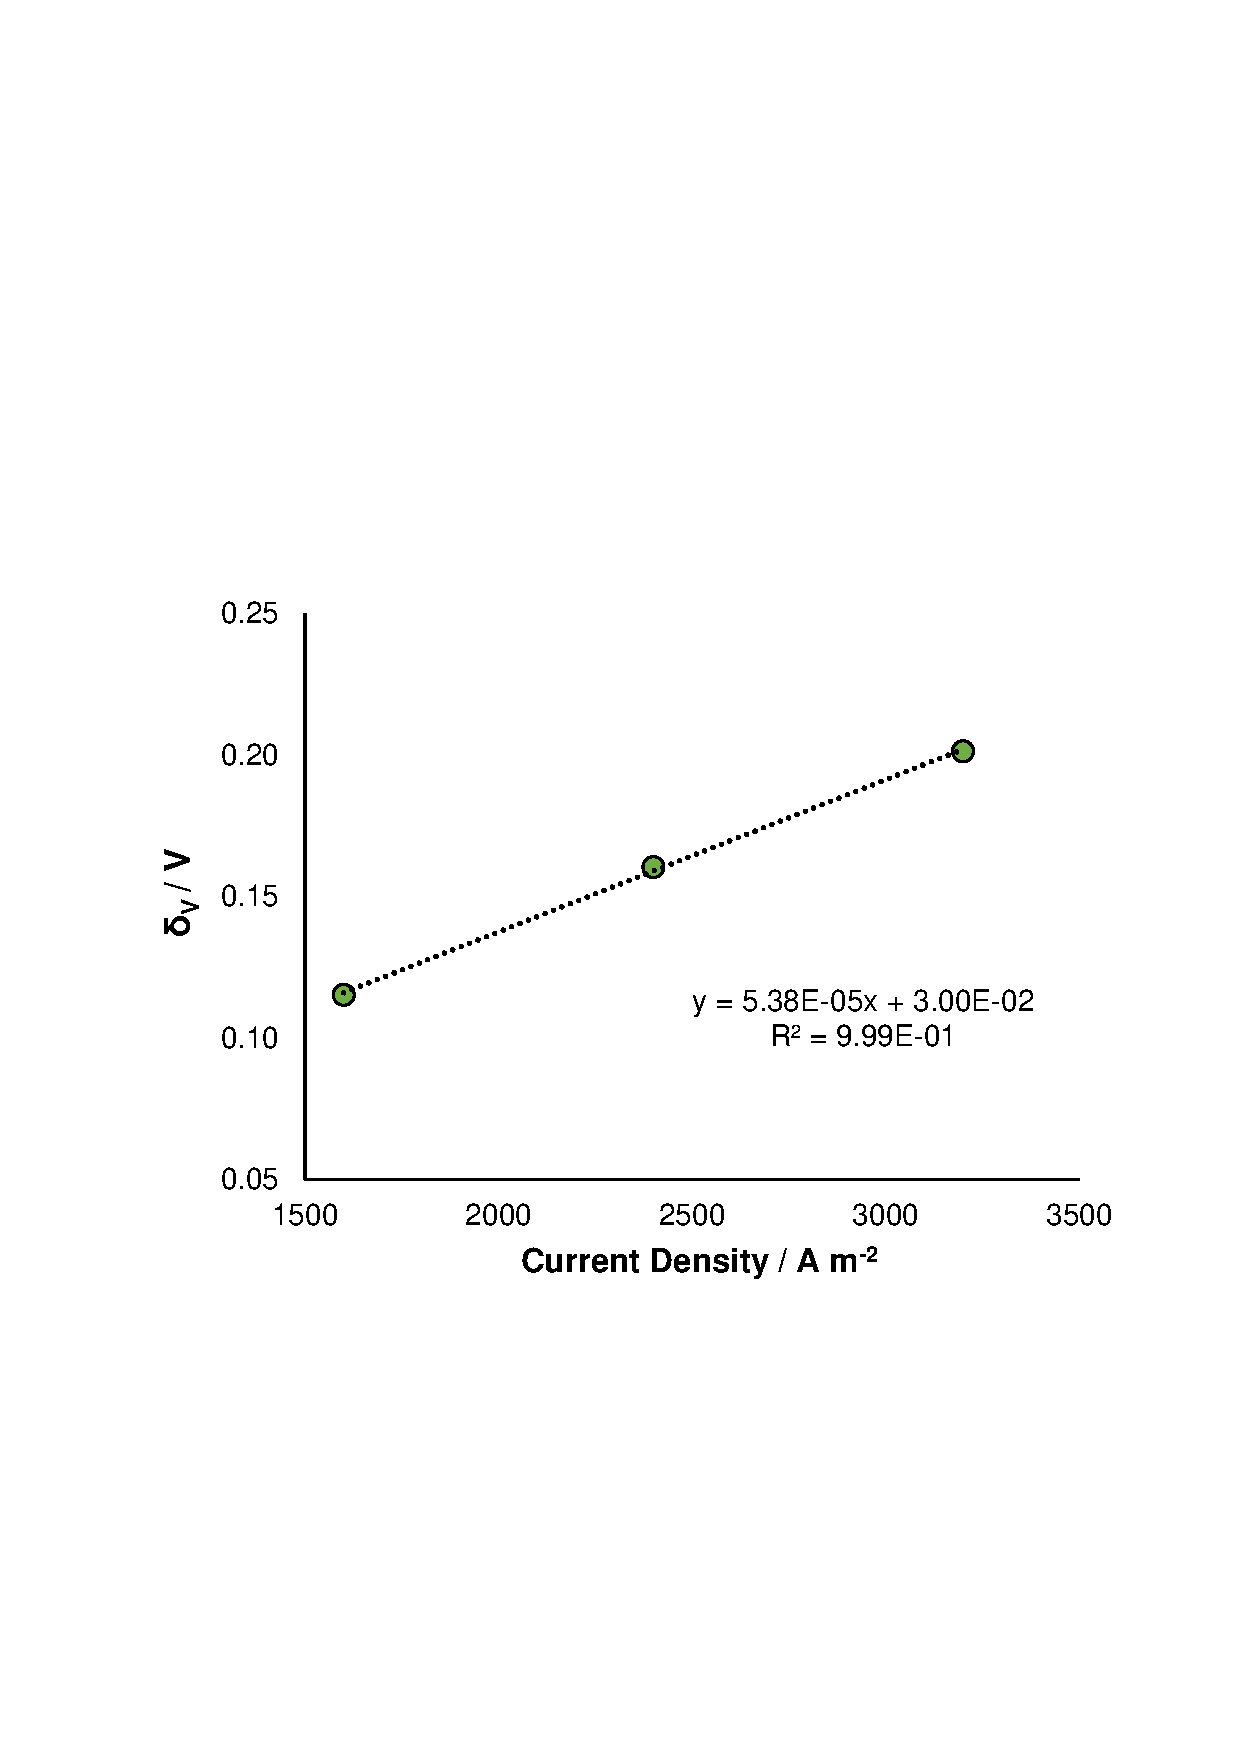
\includegraphics[trim = 2cm 8cm 2cm 9cm, clip, width = .5\textwidth]{./ASR_deriv.pdf}
\caption{Derivation of $ASR$ (gradient) and $V_a$ (intercept) for IDD2s VRFB embodiment reported by \cite{Reed2016} at 400 \si{\ml\per\minute}.}
\label{fig:Va_ASR_Derivation}
\end{figure}

The optimisation of scheduling was performed for each day in 2017 using both the NLP formulation and the LP benchmark. \Cref{fig:IDD2s_opt_schedules} shows the optimal hourly schedule determined by each method for the 22\textsuperscript{nd} of August (this date was chosen because the resultant revenue is the median of the range obtained across the year).

\begin{figure}[!ht]
\centering
\subfloat[][]{
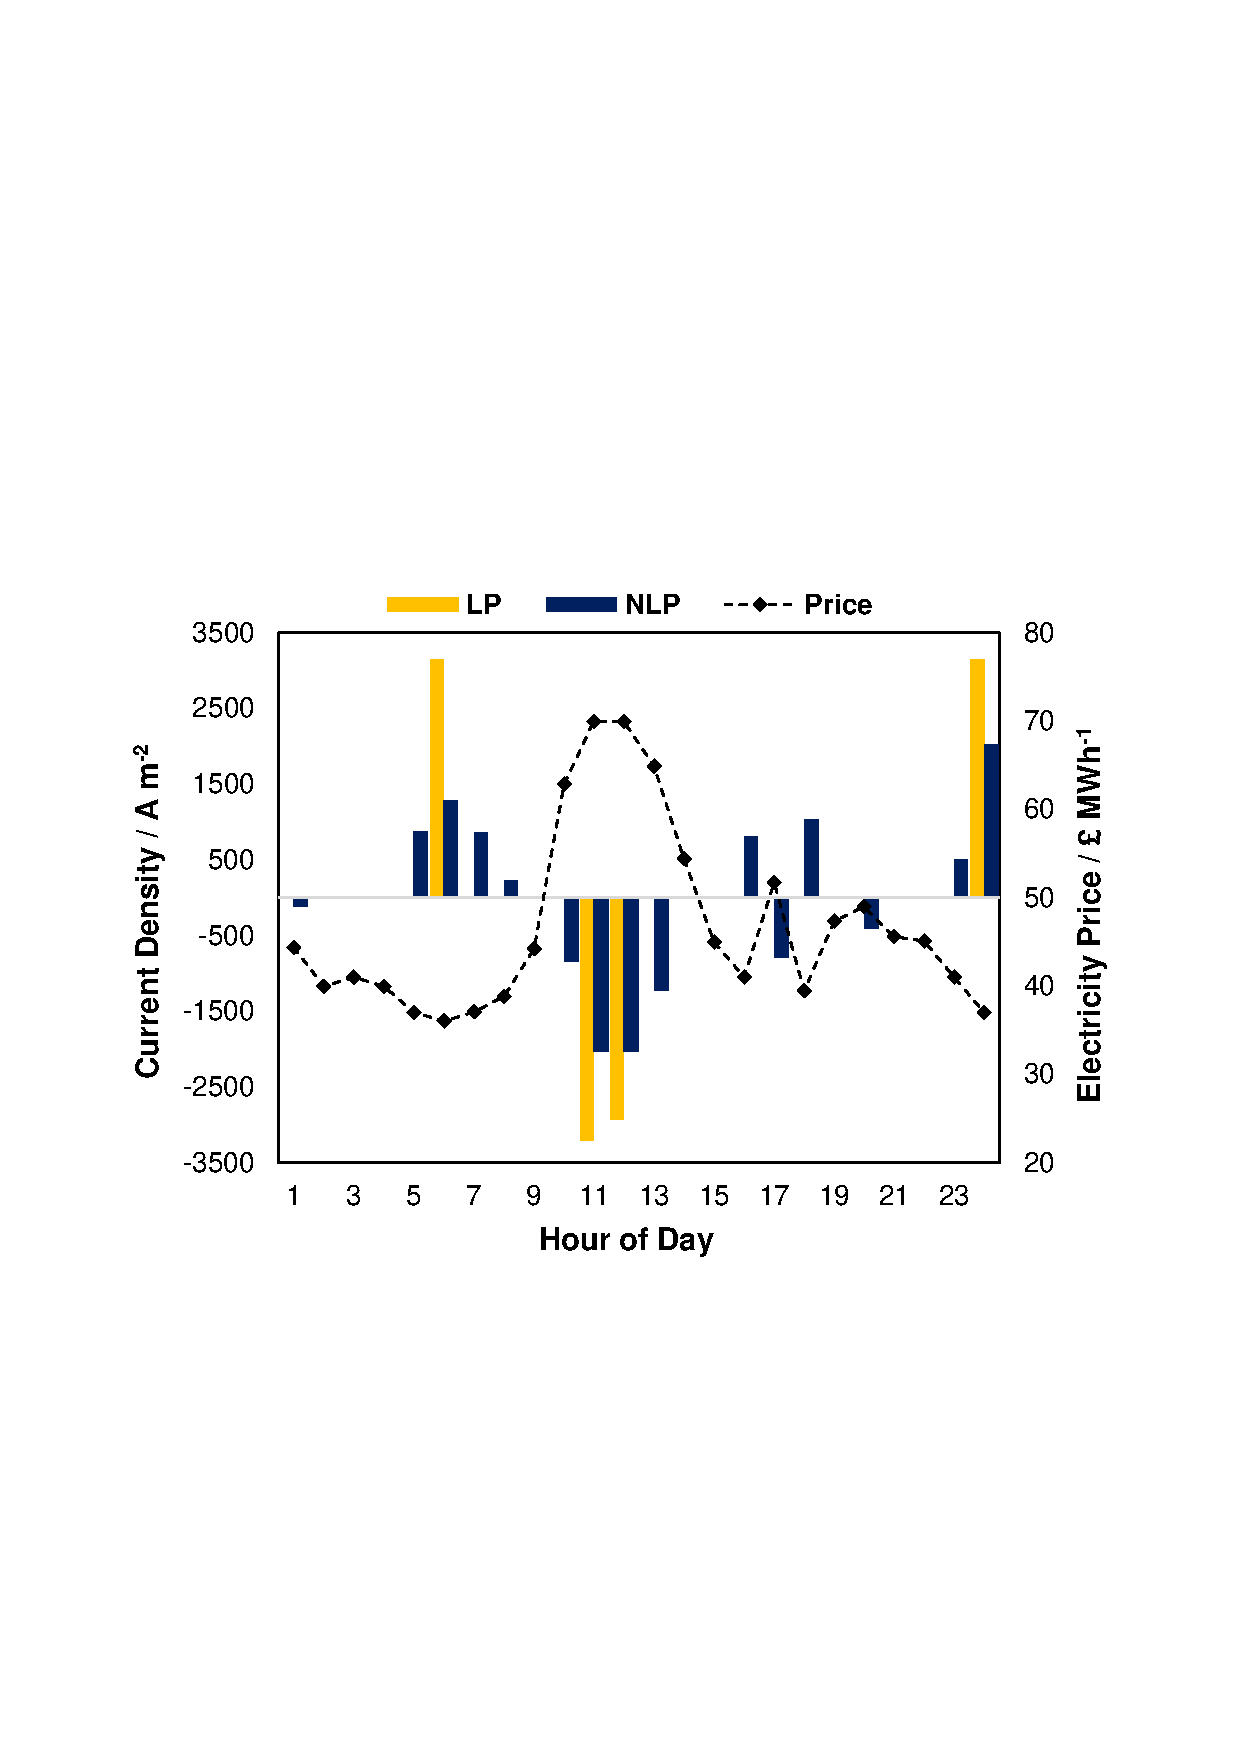
\includegraphics[trim = 2cm 8cm 2cm 9cm, clip, width = .5\textwidth]{./IDD2s_schedules.pdf}
\label{fig:IDD2s_opt_schedules}
}
\subfloat[][]{
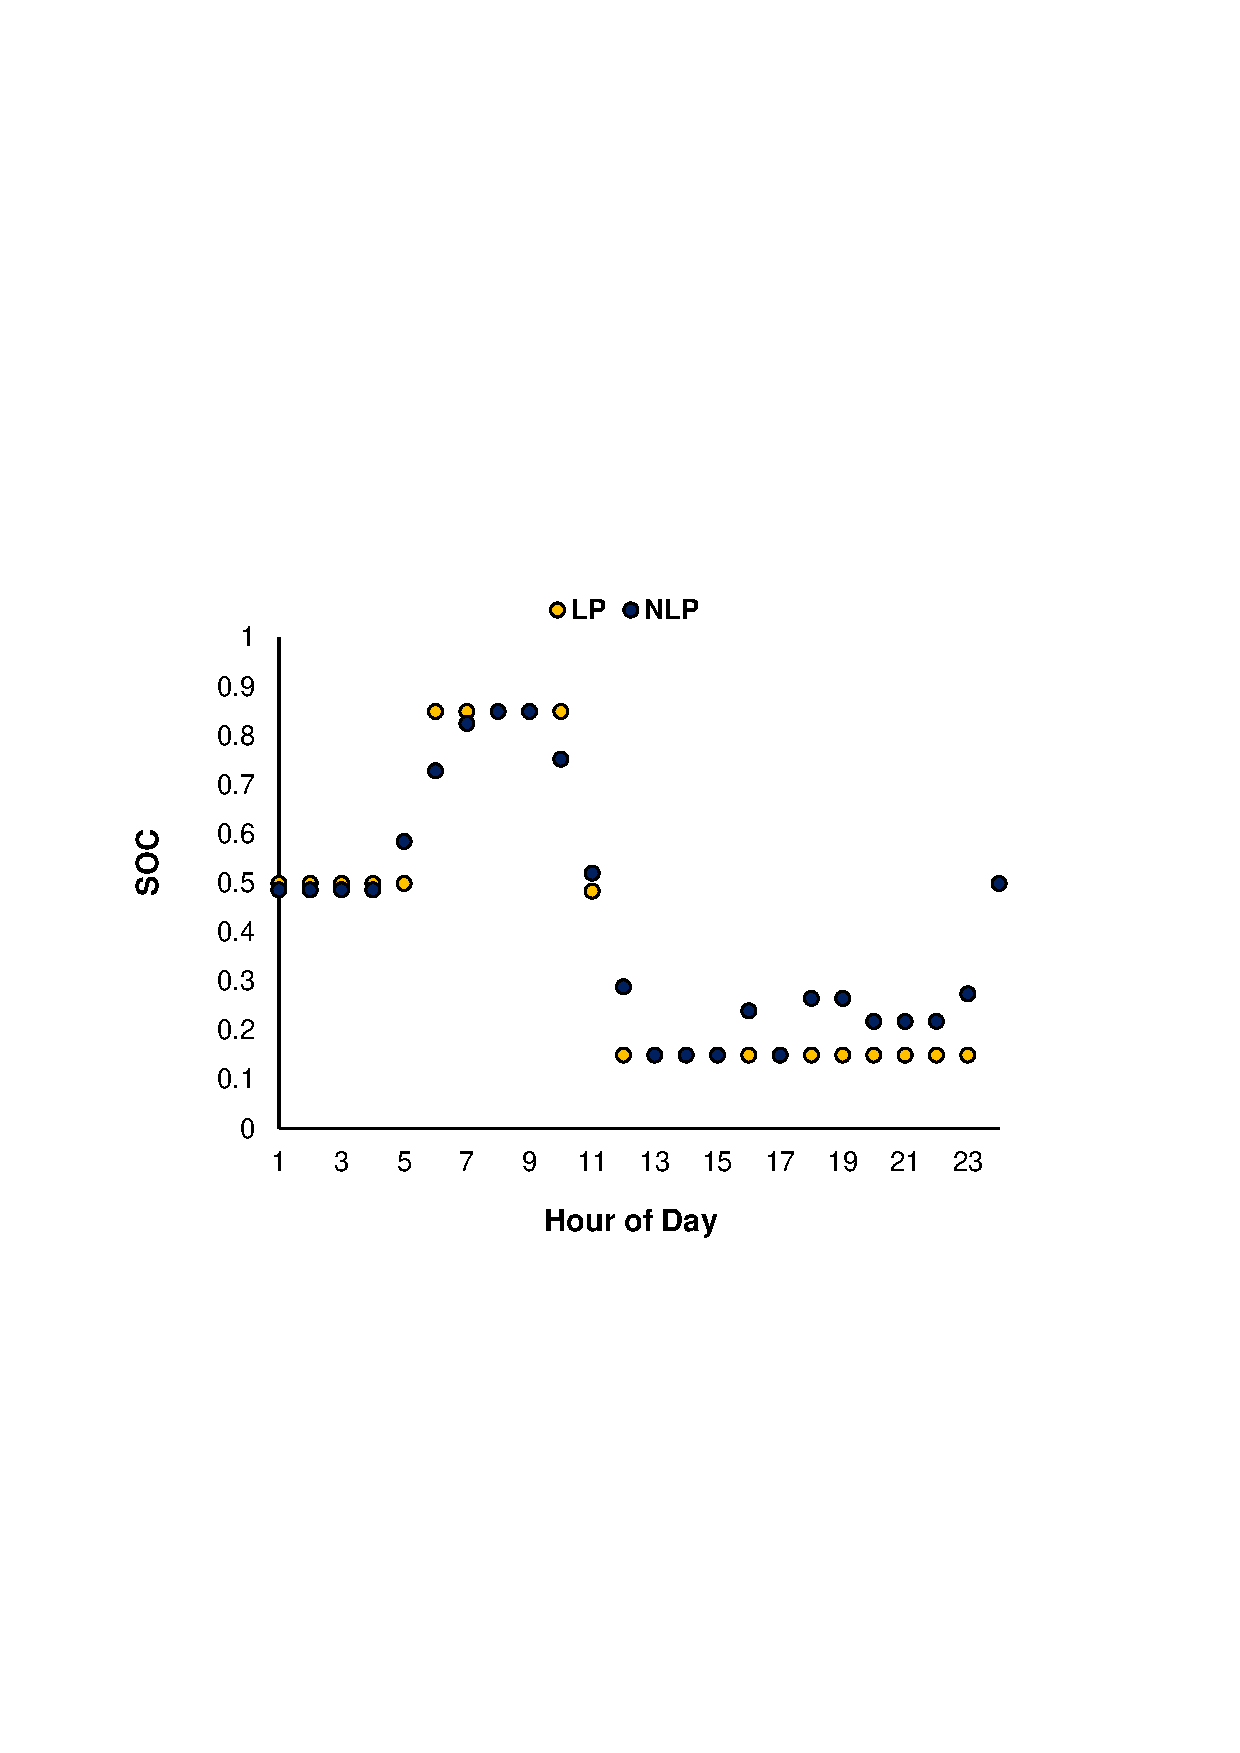
\includegraphics[trim = 2cm 8cm 2cm 9cm, clip, width = .5\textwidth]{./IDD2s_schedules_SOC.pdf}
\label{fig:IDD2s_opt_schedules}
}
\caption{(a) Optimal VRFB schedules derived for the 22\textsuperscript{nd} August 2017 using LP and NLP optimisation formulations (discharge plotted as negative). (b) corresponding SOC values.}
\end{figure}

Both the LP and NLP solutions involve charging the VRFB when the electrical price is low (e.g. between 05:00 and 07:00) and discharging it when the price is high (e.g. 10:00 to 13:00). The LP optimal profile involves discharging or charging the system at high current-density in the four hours with the most extreme prices. The NLP optimal schedule also targets the most extreme periods, but spreads the charging/discharging out. This is the consequence of factoring variable ohmic losses in the objective function -   high current-density is penalised by higher losses. Under the LP formulation, the VRFB is predicted to generate \pounds 0.068, whereas the NLP formulation predicts a revenue of \pounds 0.063. In reality however, the voltaic losses that would occur under the LP schedule would reduce the revenue to \pounds 0.051. Across 2017, LP scheduling would have resulted in \pounds 22.61 (against prediction of \pounds 33.16) and NLP scheduling would have yielded \pounds 27.99.

In a techno-economic analysis of this VRFB, use of the LP formulation would therefore lead to errors in calculation of revenue (in this case an overestimation). Use of the NLP formulation to determine scheduling in a practical application would result in significantly higher revenue than would the LP formulation. It would be possible to set a representative voltaic efficiency ($\bar\eta_V$) in the LP formulation such that the estimate of revenue would be closer to that of the NLP formulation, but this value cannot be known \textit{a priori}.

Solving \cref{eqn: Linear_Schedule_Objective_Function_Current_as_Variable} for each day in 2017 takes \SI{129}{\second} which is a minimal increase over the \SI{127}{\second} required to solve the LP objective function in \cref{eqn: Linear_Schedule_Objective_Function_Current_as_Variable}.


\subsection{NLP with functional OCV}
\label{Results_NLP_Functional_OCV}
In the second case study, the impact of expressing OCV as a function of SOC (and hence of the current-density variables in preceding sub-periods) was investigated. Parameters $a$ and $b$ representing the linear relationship between OCV and SOC in \cref{eqn: NLP_true_OCV_long_form} were set at 0.2667 and 1.333, after linear regression on data published by \cite{Kim2011}. 

\cref{fig:OCV_fixed_dynamic_schedules} shows a comparison of the optimal schedules obtained using the functionalised OCV formulation and the previous formulation (\cref{eqn: Non-Linear_Schedule_Objective_Function_Current_as_Variable}) where OCV is fixed at the 50\% SOC value ($OCV_{50\%}$). \cref{fig:OCV} shows the OCV in the former solution.

\begin{figure}[!ht]
\centering
\subfloat[][]{
\label{fig:OCV_fixed_dynamic_schedules}
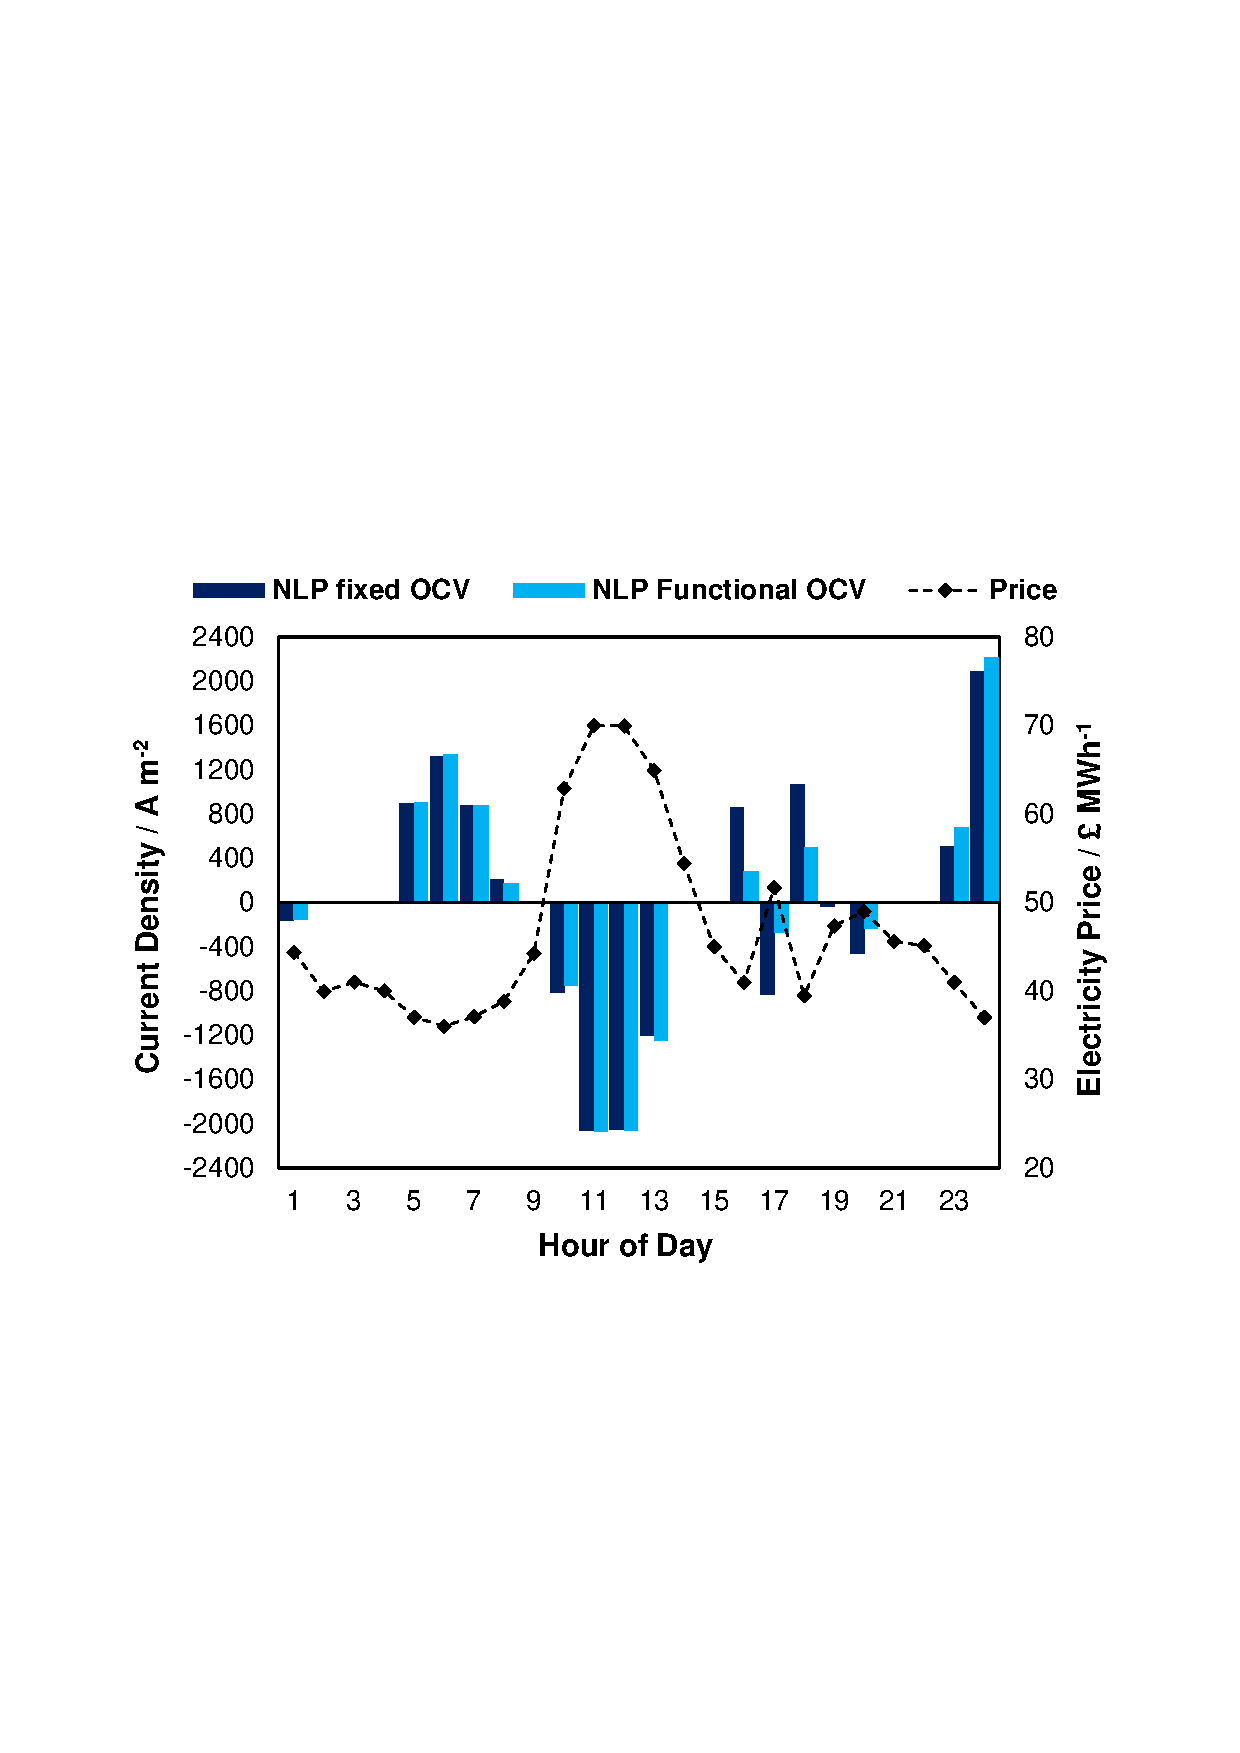
\includegraphics[trim = 2cm 8cm 2cm 9cm, clip, width = .5\textwidth]{./OCV_fixed_dynamic_schedules.pdf}

}
\subfloat[][]{
\label{fig:OCV}
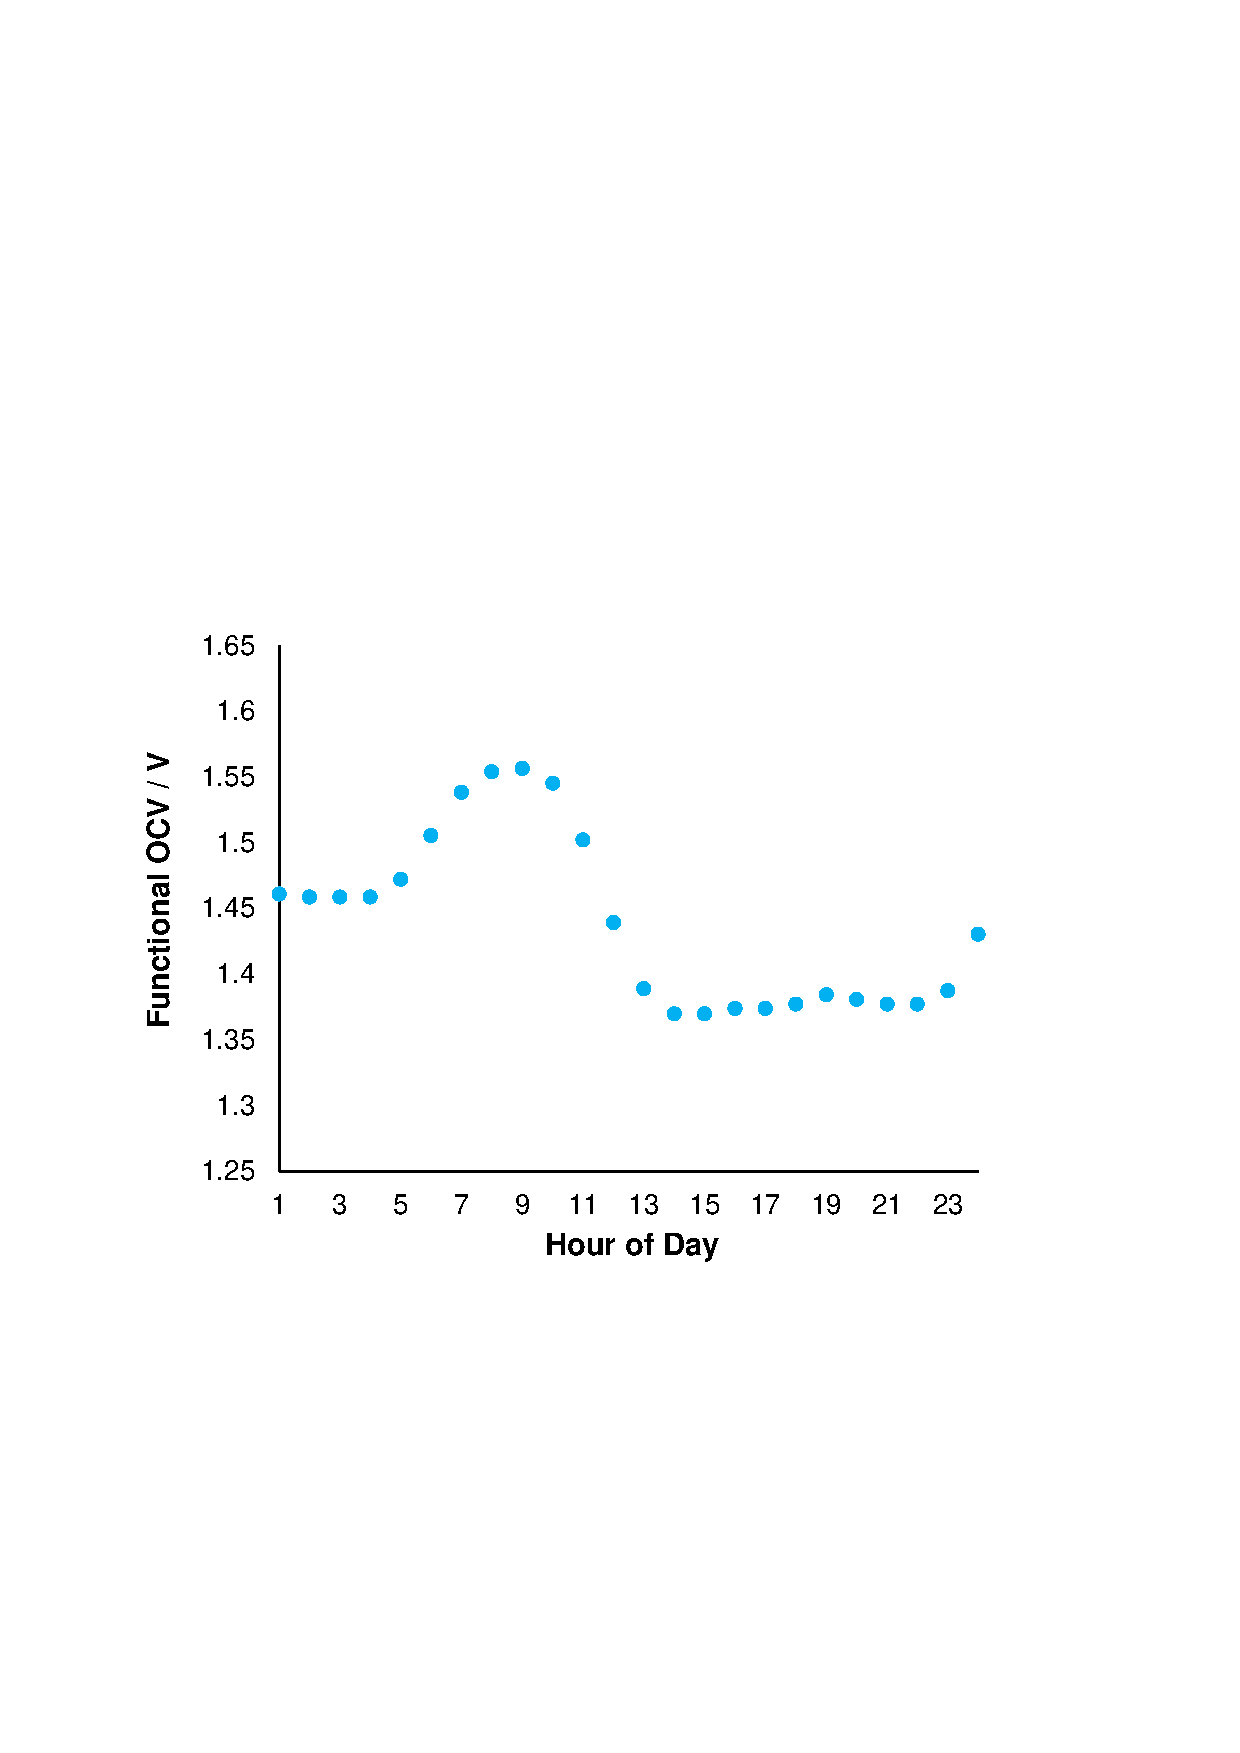
\includegraphics[trim = 2cm 8cm 2cm 9cm, clip, width = .5\textwidth]{./OCV_fixed_dynamic_OCV.pdf}
}
\caption{(a) Optimal VRFB schedules derived for the 22\textsuperscript{nd} August 2017 using NLP formulations where OCV is fixed $OCV_{50\%}$ and functionalised. (b)Optimal values of OCV where it is functionalised.}
\end{figure}

The performance of arbitrage between 16:00 and 20:00 is notably reduced when OCV is functionalised. In this period there are small fluctuations in price from which the RFB derived revenue when a fixed OCV was assumed. However the global optimum requires that the RFB be at a low SOC in these hours, and hence at a low OCV. The low OCV means that a higher current-density would be required to match the power output in the fixed OCV case, and hence higher voltaic losses would be incurred, eroding the revenue. On this date the impact on revenue is low; the optimal schedule with consideration of functional OCV results in a revenue of \pounds 0.062 compared to \pounds 0.063 for the base case. Across 2017 the formulation with functional OCV returns \pounds 26.40 compared to \pounds 27.81 for the fixed OCV case. The assumption of a fixed OCV (parametrised at 50\% SOC) therefore results in a small but not insignificant overestimation of revenue in this application. Including functionalised OCV in the objective function increases the solve time - the 2017 data were processed in \SI{217}{\second} compared to \SI{129}{\second} for the convex objective function in \cref{eqn: Non-Linear_Schedule_Objective_Function_Current_as_Variable}. 

The non-convex objective function in \cref{eqn: NLP_true_OCV_long_form} makes the formulation less robust: in the 2017 data there were two days in which the price parameter set yielded problem matrices that required greater diagonal adjustment than the default maximum permitted value of 1e-6. In these instances Gurobi returns an error message describing the diagonal adjustment that would be required. Solutions for the two days were obtained by increasing the Gurobi Parameter "PSDTol" to 1.7e-6.

\subsection{Cell-Voltage constraint}
\label{Results_Cell_Voltage_Constraint}
In the NLP formulations given in \cref{eqn: Non-Linear_Schedule_Objective_Function_Current_as_Variable,eqn: NLP_true_OCV_long_form} it is assumed that the RFB may be charged at maximum current-density at the maximum SOC. This was the charging strategy applied in \cite{Reed2016}, where the cell-voltage was allowed to reach \SI{1.85}{\volt} at the highest current-density, corresponding to an approximate SOC of 0.85. Overcharging may lead to oxygen evolution at the cathode and hydrogen evolution at the anode. This results in reduced coulombic efficiency and  (more importantly) the evolved gases can cause a range of problems as described by \cite{Kear2012}.  The particular cell-voltage at which gas evolution becomes problematic will vary from system to system (as it depends on the particular electrolyte chemistry). In this case study $V_{max}$ in \cref{eqn: Cell_Voltage_Constraint} was set at 1.65, just below the voltage at which \cite{Wei2017} reported evolution of macroscopic bubbles of hydrogen and oxygen (\SI{1.70}{\volt}). 

Maximising \cref{eqn: NLP_true_OCV_long_form} subject to \cref{eqn: Cell_Voltage_Constraint} for the 2017 data resulted in \pounds 26.07 compared to \pounds 26.40 when the cell voltage was not constrained. The difference is small because high current-density is already discouraged by the functionalised voltaic losses in \cref{eqn: NLP_true_OCV_long_form}. \cref{fig:V_max_schedules} shows the optimal schedules with and without constraint for 5\textsuperscript{th} February 2017, where the difference in revenue was greatest (\pounds 0.018 vs. \pounds 0.020). \cref{fig:V_max_voltages} shows the corresponding cell-voltage profiles.

\begin{figure}[!ht]
\centering
\subfloat[][]{
\label{fig:V_max_schedules}
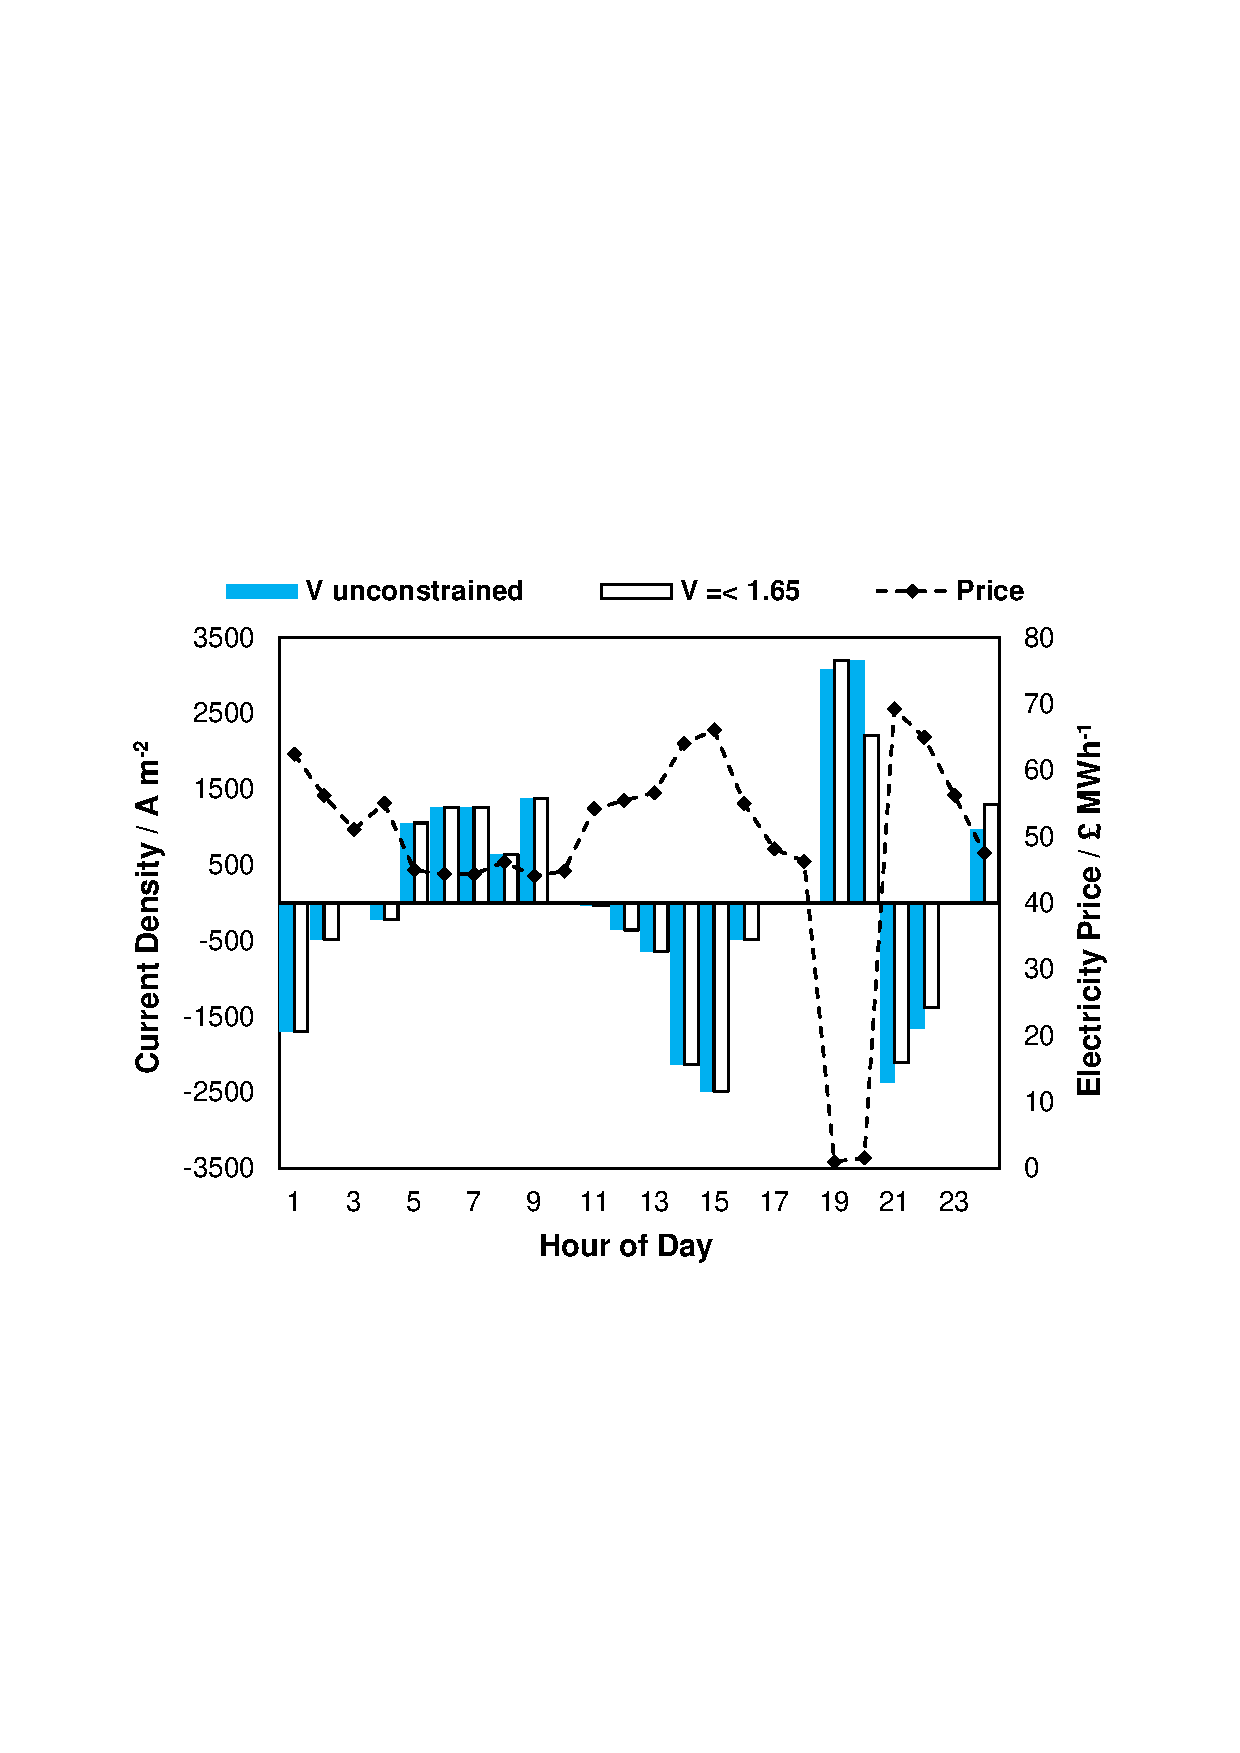
\includegraphics[trim = 2cm 8cm 2cm 9cm, clip, width = .5\textwidth]{./V_max_schedules.pdf}
}
\subfloat[][]{
\label{fig:V_max_voltages}
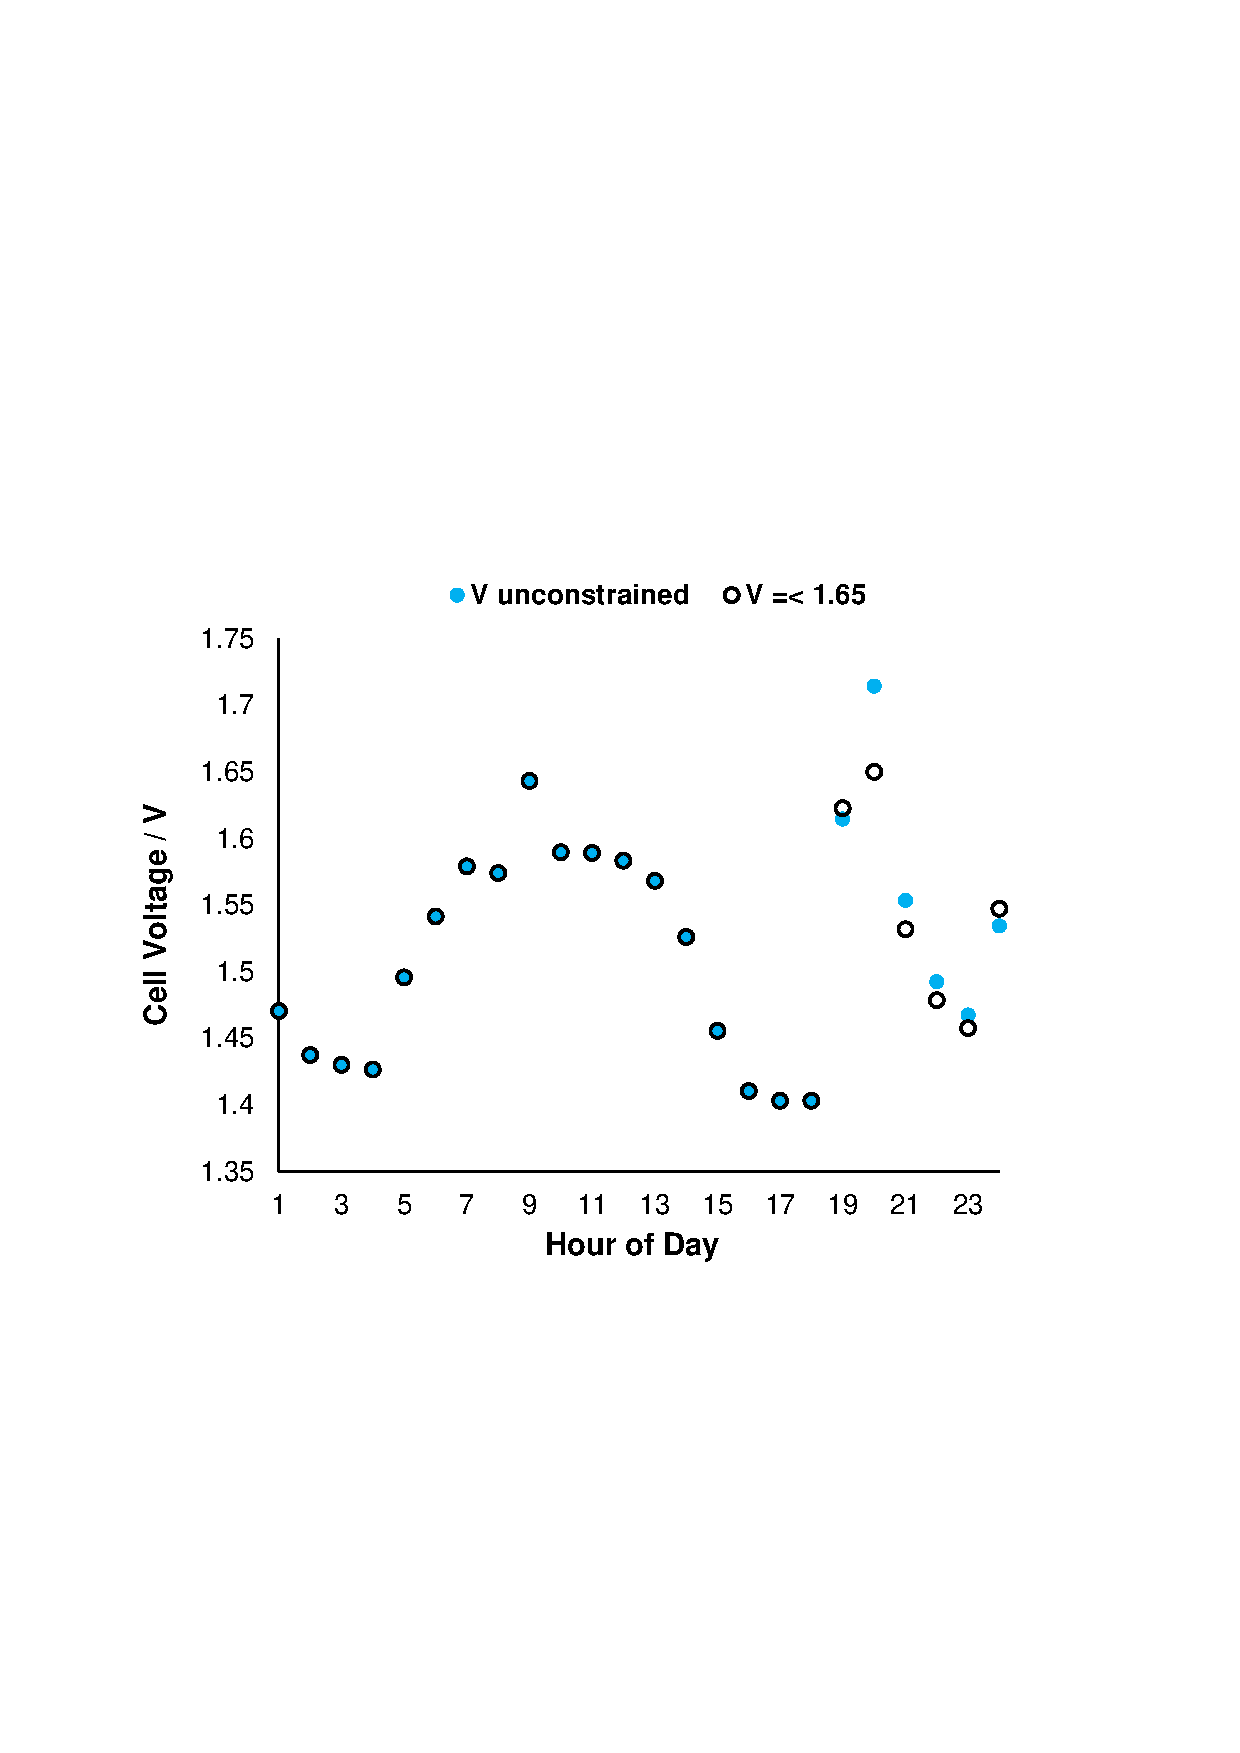
\includegraphics[trim = 2cm 8cm 2cm 9cm, clip, width = .5\textwidth]{./V_max_voltages.pdf}
}
\caption{(a) Optimal VRFB schedules derived for the 5\textsuperscript{th} February 2017 by maximising \cref{eqn: NLP_true_OCV_long_form} with no cell-voltage constraint, and subject to the cell voltage constraint given in \cref{eqn: Cell_Voltage_Constraint}. (b)Corresponding cell-voltage profiles.}
\end{figure}

In the unconstrained case the RFB charges at the maximum current-density of \SI{3200}{\ampere\per\square\meter} in hour 19 in order to capitalise on the unusually low electrical price, resulting in a cell-voltage of \SI{1.71}{\volt}. In the constrained case, the current-density is restricted to \SI{2213}{\ampere\per\square\meter} in the same period, and the RFB must charge more (and discharge less) in other periods to satisfy \cref{eqn: Method_Constraint_E_Conservation}. The impact of the constraint would be more severe if the variations in price data were greater, or the maximum voltage set at a lower value.

The application of the linear constraint on cell-voltage increases the time to process the 2017 data from \SI{217}{\second} to \SI{232}{\second}.

\subsection{Analysis of Assumptions}
\label{analysis_of_assumptions}
A number of assumptions have been made in the preceding NLP formulations in current-density terms:

\begin{enumerate}

    \item It is assumed that both coulombic efficiency and the voltaic loss parameters are invariant with SOC and symmetrical (i.e. the same for charge and discharge). Regarding the first assumption, experimental work by \cite{Nguyen2014} showed that the voltaic discharge efficiency is lower at 70\% SOC than at 35\% SOC, but that the difference decreases as power increase (data are only reported up to \SI{1.8}{\kilo\watt} for a \SI{5}{\kilo\watt} system). Regarding the latter, the same authors provide experimental evidence that the voltaic efficiency of the particular VRFB is higher for charge than discharge. The latter issue could be dealt with in the present formulation (if experimental data were made available) by including applying separate $ASR$, $V_a$ and $\eta_{C}$ terms for charge and discharge. The former issue would be more difficult to deal with, and a first step would be to perform a sensitivity study based on relevant system data.
    
    \item Coulombic efficiency is assumed to be constant with current-density, i.e. the coulombic losses are proportional to the useful current-density. This assumption fits the data reported by \cite{Reed2016}, but the behaviour below \SI{1600}{\ampere\per\square\meter} was not reported. In principle shunt current losses are a proportional to cell-voltage (as described by \cite{Xing2011}, and hence a function of SOC and over-voltage (via \cref{eqn: Cell_Voltage_Constraint}). The dependence of coulombic losses on current-density is therefore weaker than implied by the present assumption. As a first approximation, this function could be simplified to a fixed term.
    
    \item Balance of plant losses are fixed as a proportion of current-density in \Cref{eqn: Non-Linear_Schedule_Objective_Function_Current_as_Variable}, reflecting an assumption of a continuously variable pump. This neglects the increase in pressure drop with electrolyte flow (shown in \cite{Reed2016}). The formulation may be improved by removing the $(1-l_{BOP})$ terms and adding a quadratic function of current-density. Alternatively the pump may have a  fixed output and be sized such that the maximum charge/discharge current-density may be satisfied at the highest/lowest SOC without incurring a significant additional over-potential due to mass-transport limitations.
    
    \item The RFB is not thermally constrained. The VRFB based on a sulphate electroylte is liable to precipitation of  V\textsubscript{2}O\textsubscript{5} from the catholyte as temperature increases (\cite{Rahman2009,Vijayakumar2011}). Although the chloride and mixed acid electrolytes developed at PNNL are more stable (\cite{Li2011,Kim2011}), temperature remains an important consideration. The framework introduced here could easily be expanded to capture the thermal performance of the system. A thermal constraint could be put in place using a similar construct to the one describing SOC, where the increase of heat in the electrolyte in sub-period $t$ is equal to the ohmic losses ($(I_{D,t}^{2} + I_{C,t}^{2})ASR$). This would allow cost benefit analyses of active cooling versus restrictions on operation at different electrolyte concentrations.

    
\end{enumerate}

As discussed above, both the coulombic losses and the pumping power may be better represented as fixed terms. In this case, the efficiency of the system at low power input/output will be unfavourable (as demonstrated by \cite{Nguyen2014}). An issue with representing these losses as fixed terms, is that they would be present at all times in the schedule. In order to minimise parasitic losses, a binary "on/off" variable could be added to the formulation in order to allow idling.

\section{Conclusion} 
\label{sec:Conclusion}
A novel framework for RFB schedule optimisation has been introduced in which the voltaic and coulombic components of the power output/input are separated, with the problem variablised in terms of current-density. An arbitrage case-study is used to demonstrate the increased fidelity that is achievable using the framework.

The framework is first used to describe ohmic losses as a quadratic function of current-density in the objective function, hence maintaining a convex solution space and all linear constraints. The importance of inclusion of variable ohmic losses in the arbitrage case study if demonstrated. Optimal deterministic scheduling using the introduced formulation (NLP) resulted in 24\% greater revenue across 2017 when compared to a basic LP approach that assumes a constant representative voltaic efficiency. In the context of a TEA, failure to factor in the variable voltaic losses leads to an overestimation of revenue by 47\%. The improved NLP treatment of voltaic losses only requires a minimal increase in computing time when compared to the LP problem with fixed voltaic efficiency. 

The framework also facilitates the expression of OCV as a function of SOC, rather than assuming a fixed average value. The non-convex objective function that results may be solved using Gurobi, although there is a penalty in computing time. For the arbitrage case study, it is demonstrated that assuming a fixed OCV results in a small but significant overestimation of revenue. This assumption should be checked for other applications.

The framework also allows for an additional linear constraint to be placed on upper cell-voltage as a function of SOC and over-potential. This constraint restricts the current-density at which the battery may be charged when the SOC is high, which is an important consideration for safety and battery lifetime. In the present case study, the impact of the chosen maximum voltage is low, as the previous factoring of voltaic losses already discourages high power input. However, in applications with greater price variation this constraint will become more important. 

A number of improvements to the particular problems presented are proposed, in order to more faithfully represent coulombic losses, the parasitic consumption of power in electrolyte pumping, and to allow idling.

It is intended that the novel framework be used for techno-economic analysis and optimisation of various RFB chemistries at a system level (i.e. up to the AC-DC boundary), for example in the optimal specification of pump rating, or cooling system for a particular application. RFB systems have previously been the subject of technical optimisation, for example the study of the trade-offs between electrolyte concentration and ASR (\cite{Weber2013} \emph{this should be weber et al.}), or shunt currents and pumping losses (\cite{Viswanathan2014}. In these works, a simple metric such as levelised cost of electrical energy under a simple duty cycle is used as the objective to minimise. The framework introduced here allows optimisation in terms of revenue under optimal scheduling for any application where a price signal exists.

Although the framework was conceived with RFB systems in mind, the easy application of a cell-voltage constraint would be useful for Li-ion scheduling, where low and high cell-voltages increase cell degradation, and the latter also poses a safety concern. In the case of Li-ion batteries, where coulombic losses are negligible, the present assumption of a fixed coulombic efficiency would be entirely appropriate. The introduced treatment of voltaic losses is an improvement over that of \cite{Sarker2017} as the constraints are all linear.

\section{Acknowledgements}

This work was supported by the UK Engineering and Physical Science Research Council via grant EP/L016818/1 which funds the Centre for Doctoral Training in Energy Storage and its Applications. Drax?


\section*{References}
\bibliographystyle{elsarticle-harv}
\bibliography{Elsevier_article.bib}


\end{document}
